
\newif\ifTODO\TODOtrue                        % Use todo notes?

%===============%                               %~~~~~~~~~~~~~~~~~~~~~~~~~~~~~~~~~~~~~~~~~~~~~~~~~%
% DOCUMENTCLASS %                                See full option description in "mytemplate.cls"
%===============%                               %~~~~~~~~~~~~~~~~~~~~~~~~~~~~~~~~~~~~~~~~~~~~~~~~~%
 
\documentclass[
a4paper,10pt
]{common/ica2013_2}

\usepackage[utf8x]{inputenc}
\usepackage[table,dvipsnames,svgnames]{xcolor}
\usepackage{titlesec}

\newcommand\Fig[1]{Fig. \ref{#1}}

\newcommand\Grey[1]{{\color{Grey}#1}}
\newcommand\Red[1]{{\color{Red}#1}}
\newcommand\Blue[1]{{\color{Blue}#1}}
\newcommand\DarkBlue[1]{{\color{DarkBlue}#1}}
\newcommand\LightBlue[1]{{\color{LightBlue}#1}}
\newcommand\Brown[1]{{\color{Brown}#1}}
\newcommand\Green[1]{{\color{Green}#1}}
\newcommand\SeaGreen[1]{{\color{SeaGreen}#1}}
\newcommand\Yellow[1]{{\color{yellow}#1}}
\newcommand\Orange[1]{{\color{orange}#1}}

\ifTODO
   \newcounter{todoidx}
   \definecolor{todobackground}{rgb}{0.95,0.95,0.95}
   \setlength\marginparsep{1pt}
   \setlength\marginparwidth{35pt}
   \newlength\marginparwidthsmall
   \setlength\marginparwidthsmall{\marginparwidth}
   \addtolength\marginparwidthsmall{-7pt}
   \newcommand\todo[1]{%
      \addtocounter{todoidx}{1}%
      {\color{Red}\bf(\thetodoidx{})}%%\fbox{\bf\thetodoidx{}}}%
      \marginpar{%
         {\vspace*{-10pt}\color{Red}\fbox{\bf\thetodoidx{}}}\\%
         \fcolorbox{red}{todobackground}{\parbox{\marginparwidthsmall}{\scriptsize #1}}}}

   \newcommand\todopar[1]{\fcolorbox{red}{white}{\parbox{0.97\linewidth}{#1}}}
\else
%    \usepackage[disable]{./todonotes} 
   \newcommand\todo[1]{}
\fi

\newcommand\nn{\nonumber\\}

\newcommand\nmat[1]{\begin{matrix}#1\end{matrix}}
\newcommand\bmat[1]{\begin{bmatrix}#1\end{bmatrix}}
\newcommand\case[1]{\begin{cases}#1\end{cases}}
\newcommand\textbox[2]{\footnotesize\text{\parbox{#1}{\centering\emph{#2}}}}

\newcommand\rand{\text{rand}}
\newcommand\randn{\text{randn}}
\newcommand\rect{\text{rect}}
\newcommand\sinc{\text{sinc}}
\newcommand\tr{\text{tr}}
\newcommand\adj{\text{adj}}

% \newcommand\max{\text{max}}
\newcommand\argmin[1]{\text{arg}\,\underset{#1}{\text{min}}}

\newcommand\qqquad{\quad\qquad}
\newcommand\qqqquad{\qquad\qquad}

\renewcommand\l[1]{\left#1}
\renewcommand\r[1]{\right#1}

% {\text{\parbox{1.5cm}{\centering volume hyper- sphere}}}

%Keyword colouring:
\newcommand\kw[1]{#1}
\newcommand\parm[1]{#1}%\color{Black}#1\color{Black}}

\newcommand\of[1]{\scriptstyle(\parm{#1})\displaystyle}
\newcommand\df[1]{\scriptstyle[\parm{#1}]\displaystyle}
\newcommand\var[3]{#1_\text{#2}\of{#3}}

\newcommand\diag{\text{diag}}

% \raisebox{lift}[extend-above-baseline][extend-below-baseline]{text}
\newcommand\mt[1]{\text{\emph{#1}}} %mt = mathtext
\newcommand\mathnorm{\textstyle}
\newcommand\mathbig[1]{\displaystyle#1\mathnorm}
\newcommand\mathsmall[1]{\scriptstyle#1\mathnorm}
\newcommand\mathtiny[1]{\scriptscriptstyle#1\mathnorm}
\newcommand\sfrac[2]{\scriptstyle\raisebox{0.25pt}[0pt][0pt]{$\frac{#1}{#2}$}\mathnorm}
\newcommand\nfrac[2]{\textstyle\frac{#1}{#2}\displaystyle}

\newcommand\sumu[1]{\sum\limits^{#1}\,}
\newcommand\suml[1]{\sum\limits_{#1}\,}
\newcommand\sumb[2]{\sum\limits_{#1}^{#2}\,}

\newcommand\produ[1]{\prod\limits^{#1}\,}
\newcommand\prodl[1]{\prod\limits_{#1}\,}
\newcommand\prodb[2]{\prod\limits_{#1}^{#2}\,}

\newcommand\defeq{\overset{\underset{\mathrm{def}}{}}{=}}

%Math macros:
\newcommand\diff[2]{\frac{\kw{d}\,\textstyle #1\scriptstyle}{\kw{d\parm{#2}}}\displaystyle}
\newcommand\ddiff[2]{\frac{\kw{d^2}\,\displaystyle #1\scriptstyle}{\kw{d\parm{#2}}^2}\displaystyle}

\renewcommand\d[1]{\scriptstyle\kw{\,d\parm{#1}}\displaystyle}

% These commands are mutually exclusive. Remember to "renew" in v2.
\newcommand\intb[4]{\int\limits_{#3}^{#4} #1 \d{#2}} % \int{exp}{var}{from}{to}
\newcommand\intl[3]{\int\limits_{#3} #1 \d{#2}} % \int{exp}{var}{for all}
\newcommand\intu[2]{\int #1 \d{#2}} % \int{exp}{var}{for all}

\newcommand\T{^{\scriptscriptstyle T}}
\renewcommand\H{^{\scriptscriptstyle H}}

\renewcommand\vec[1]{\boldsymbol{#1}}
\newcommand\mat[1]{\boldsymbol{#1}}

\newcommand\1{\vec 1}
\newcommand\I{\mat I}
\renewcommand*\a{\vec a}
\renewcommand*\i{\vec i}
\renewcommand*\k{\vec k}
\newcommand*\n{\vec n}
\newcommand*\p{\vec p}
\newcommand*\s{\vec s}
\newcommand*\w{\vec w}
\newcommand*\x{\vec x}
\newcommand*\y{\vec y}

\newcommand*\A{\mat A}
\newcommand*\B{\mat B}
\newcommand*\C{\mat C}
\newcommand*\E{\mat E}
% \renewcommand*\H{\mat H}
\renewcommand*\P{\mat P}
\newcommand*\eP{\mat{\hat P}}
\newcommand*\R{\mat R}
\newcommand*\Ri{\R^{-1}}
\newcommand*\eR{\mat{\hat R}}
\newcommand*\eRi{\hat{\mat R}\,\!^{-1}}
\newcommand*\Navg{N_\text{avg}}
\newcommand*\W{\mat W}
\newcommand*\X{\mat X}
\newcommand*\Xd{\X_{\!\Delta}}
\newcommand*\Y{\mat Y}

\renewcommand*\L{\mat \Lambda}
\newcommand*\U{\mat U}
% \renewcommand*\t{\mathtiny{^T}}
% \newcommand*\h{\mathtiny{^H}}
\renewcommand*\t{^T}
\newcommand*\h{^H}

\newcommand\D{\vec\nabla} %Del: Vector differential operator - nabla
\newcommand\Dx{\vec\nabla\times}
\newcommand\Dd{\vec\nabla\cdot}

\usepackage{tikz}
\usetikzlibrary{shapes,snakes}
\usepackage{amsmath,amssymb}
\usepackage{glossaries}

\newenvironment{outline}
{\begin{itemize}}
{\end{itemize}}


\begin{document}
% \setlength{\headrulewidth}{0.0pt}

%~~ TitlePage ~~%                               %~~~~~~~~~~~~~~~~~~~~~~~~~~~~~~~~~~~~~~~~~~~~~~~~~%
\thispagestyle{empty}
\pagenumbering{arabic} %Normal numbers


{\Large\bf Adapting the MVDR beamformer to a GPU for differently sized active sonar imaging systems.}

\begin{abstract}
The MVDR beamformer has been shown to improve active sonar image quality compared to conventional methods. Unfortunately, it is also significantly more computationally expensive because a spatial covariance matrix must be estimated and inverted for each image pixel. We target this challenge by altering and mapping the MVDR beamformer to a GPU, and suggest three different solutions depending on the system size.

For systems with relatively few channels, we suggest arithmetic optimizations for the estimation step, and show how a GPU can be used to yield image creation rates of more than 1\,Mpx/s. For larger systems we show that frequency domain processing is preferable, as this promotes high processing rates at a negligible reduction in image quality. These GPU implementations consistently reduced the runtime by 2-3 orders of magnitude compared to our reference C and Matlab implementations.

For even larger systems we suggest employing the LCA beamformer. It does not calculate a weightset, but merely computes the beamformer output for each of a predefined set of weights, and selects the one that best fulfils the MVDR criterion. The LCA creates images with a quality comparable to MVDR, and it is perfectly suited for a GPU.

\ \\
Total: 195 words (200 max)

\ \\
Noen tanker jeg har selv naa:
\begin{itemize}
\item Det mangler noe om bruksomraader.
\item Maa passe paa aa ikke selge LCA saa bra at MVDR ser helt haaplos ut(?)
\item 200 ord er ingenting. :)
\end{itemize}


\ \\
Questions they wanted answered:
\begin{itemize}
\item This session will feature work on adapting computationally demanding modeling and signal processing tasks to take advantage of various parallel architectures, such as cloud computing, computing clusters, multicore CPUs, multi-core graphic processing units (GPUs), DSP chips, and FPGAs.
\item If algorithm is slow - What technology will help me?
\item What skills are needed?
\item What tools are available and what's the cost?
\item What acceleration factor are we looking at?
\item How can I get started?
\item What we did. Which tools? Was it hard? Speedup?
\end{itemize}
\end{abstract}

\section{Introduction}

To improve the image quality active sonar imaging several data adaptive techniques have 

Most modern active sonar imaging systems operate by combining data from sensor arrays to , from which data is combined 

The Minimum Variance Distortionless Response (MVDR) beamformer is known for its potential to improve sonar image quality. 

Most active sonar systems today employ phased arrays to record and 

Adaptive beamforming have in recent years been applied to active sonar imaging by several authors. 

The potential that adaptive beamformers to improve active sonar image quality is  ers is that theimprove image quality by utilising the apriori knowledge present in the backscattered wavefield.  has for improving active sonar image quality has been demonstrated in e.g. []. are known for the potential to improve image quality in to When using adaptive beamformers to improbe

\section{Methods}

Suppose that a backscattered wavefield is recorded by an $M$ element uniform linear array, and let the output from the $m$'th channel be given as $x_m$. By definition a beamformer's output $z$ is a weighted sum $z$ of all these data outputs:
\begin{align}
z[n] = \w\H[n]\x[n] = \bmat{w_0[n]\\w_1[n]\\\vdots\\w_{M-1}[n]}^H \bmat{x_0[n]\\x_1[n]\\\vdots\\x_{M-1}[n]},\label{z}
\end{align}
where $w_m$ is the weight factor assigned to channel $m$. With static weights this would be referred to as the conventional delay-and-sum (DAS) beamformer. Various weighting patterns exists here for trading lateral resolution for improved noise suppression (contrast), but one always ends up with a compromise between the two\todo{don't quite like this one}~\cite{Harris1978}.

\subsection{MVDR beamformer}

Adaptive beamformers target this limitation by allowing the weights to change for each pixel to better fit the dynamic nature of the incoming wavefield. The MVDR beamformer is one such method. It finds the set of complex weights that minimizes the beamformer's expected output power, $\argmin{\w}\,E\{|z[n]|^2\}$, while ensuring unity gain in the look direction~\cite{Capon1969}. The solution to this optimization problem is given as:
\begin{gather}
\vec w[n] = \frac{\Ri[n]\1}{\1\T\Ri[n]\1},\label{weights}
\end{gather}
where $\1$ is a row vector of ones that represents broadside steering, and $\R=E\{\x[n]\x\H[n]\}$ is the spatial covariance matrix for the full array. Since $\R$ is unknown, we estimate it by by computing a sample covariance matrix $\eR$. In this computation we will perform some degree of \emph{spatial averaging} to avoid signal cancellation, \emph{temporal averaging} to maintain true speckle statistics, and \emph{diagonal loading} to improve robustness to parameter errors ~\cite{Synnevag2009a}. Combined, these steps will also ensure a numberically well conditioned $\eR$\todo{should we mention variance reduction?}.

If we let $x_l[n]$ represent the datavector from subarray $l$,
\begin{gather}
\x_l[n] = \bmat{x_l[n] & x_{l+1}[n] & \dots & x_{l+L-1}[n]}\T,
\end{gather}
then a sample covariance matrix formed with temporal and spatial averaging, $\eR_\text{s,t}$, is given as:
\begin{gather}
\eR_\text{s,t}[n] =  \frac{1}{N_K N_L} \sumb{l=0}{M-L}\sumb{n'=n-K}{n+K} \x_l[n]\x_l\H[n] \in\mathbb{C}^{L,L},\label{spatialR}
\end{gather}
where $N_K = 2K+1$ is the number of temporal samples to perform averaging over, and $N_L = M-L+1$ is the number of subarrays.

To further improve robustness, we add a fraction $d$ of the total power of $\eR_\text{t,s}[n]$ to its diagonal~\cite{Synnevag2007}:
\begin{align}
\eR[n] = \eR_\text{t,s}[n] + \I \frac{d}{L} \tr\{\eR_\text{t,s}[n]\},\label{finalR}
\end{align}
where $\I$ is an identity matrix, $\tr\{\cdot\}$ represents the matrix trace operation, and $\tr\{\eR_\text{t,s}[n]\}$ is an estimate of the energy received by this pixel.

\subsection{LCA beamformer}




Note how subarray averaging led to a size reduction of $\eR$ from $\mathbb{C}^{L,L}$ to $\mathbb{C}^{M,M}$, and hence will produce an $L$-element weightset when substituted into (\ref{z}). This weightset is then applied to on all the subarrays, prior to computing the beamformer output as in (\ref{z}). Or, equivalently, we may apply the weightset to the sum of all the subarrays:
\begin{align}
z[n] = \w\H[n] \sumb{l=0}{M-L} \x_l[n].\label{finalZ}
\end{align}
\begin{figure}[!t]\centering
\includegraphics[width=\linewidth]{gfx/implementation.eps}
\caption{MVDR beamforming. For one of the total number of pixels in range and azimuth, $N_y$ and $N_x$,\newline
1. an $L\times{}L$ sample covariance matrix $\eR$ is computed, \newline
2. the term $\eR^{-1}\1$ is found using a linear equation solver,\newline
3. and the beamformer output is computed from $z$ from (\ref{finalZ}), where $\w$ is found by substituting $\eR^{-1}\1$ into (\ref{weights}). } \label{mvdr_beamforming}
\end{figure}
% \begin{figure}[!t]\centering
% \includegraphics[width=\linewidth]{gfx/algorithm_structure.eps}
% \caption{MVDR beamforming. First a spatial covariance matrix is estimated from the delayed data (\ref{spatialR}-\ref{finalR}), then the weights are computed (\ref{weights}) and finally applied to the delayed channel data (\ref{z}).}
% \label{implementation}
% \end{figure}
As summarized in Fig. \ref{mvdr_beamforming}, the MVDR method is applied to each pixel independently, by
\begin{enumerate}
\item computing the sample covariance matrix $\eR$ in (\ref{finalR}),
\item computing $\eRi\1$ in (\ref{weights}), and
\item computing the beamformer output $z$ in (\ref{finalZ}).
\end{enumerate}




\section{Results}

\begin{figure}[!t]\centering
\includegraphics[width=\linewidth]{gfx/implementation.eps}
\caption{MVDR beamforming. For one of the total number of pixels in range and azimuth, $N_y$ and $N_x$,\newline
1. an $L\times{}L$ sample covariance matrix $\eR$ is computed, \newline
2. the term $\eR^{-1}\1$ is found using a linear equation solver,\newline
3. and the beamformer output is computed from $z$ from (\ref{finalZ}), where $\w$ is found by substituting $\eR^{-1}\1$ into (\ref{weights}). } \label{mvdr_beamforming}
\end{figure}



% 
% \ \\
% Total: 192 words (200 max)
% 
% \ \\
% Noen tanker jeg har selv naa:
% \begin{itemize}
% \item Det mangler noe om bruksomraader.
% \item Maa passe paa aa ikke selge LCA saa bra at MVDR ser helt haapløs ut(?)
% \item 200 ord er ingenting. :)
% \end{itemize}
% 
% 
% \ \\
% Questions they wanted answered:\cite{Kailath1985}
% \begin{itemize}
% \item This session will feature work on adapting computationally demanding modeling and signal processing tasks to take advantage of various parallel architectures, such as cloud computing, computing clusters, multicore CPUs, multi-core graphic processing units (GPUs), DSP chips, and FPGAs.
% \item If algorithm is slow - What technology will help me?
% \item What skills are needed?
% \item What tools are available and what's the cost?
% \item What acceleration factor are we looking at?
% \item How can I get started?
% \item What we did. Which tools? Was it hard? Speedup?
% \end{itemize}
% \end{abstract}

\bibliographystyle{common/jasanum}
\bibliography{../../Library/library}

% \section{Introduction}

\end{document}
